\documentclass[12pt, letterpaper, twoside]{article}
\usepackage[utf8]{inputenc}
\usepackage{graphicx}
\graphicspath{{/home/justin/mythesis/Graphics/}}
 
\title{Estimating the Electron Background}
\author{Justin Estee}
\date{August 2019}
 
\begin{document}
 
\begin{titlepage}
\maketitle
\end{titlepage}
 
 \newcommand\elec{\mathrm{e^-}}
\newcommand\postr{\mathrm{e^+}}
\newcommand\piz{\mathrm{\pi_0}}

\section{Electron background}
The $\piz$ decays through two main branches, 
\begin{equation}
\piz \rightarrow \gamma\gamma
\label{eq:branch1}
\end{equation} 
 
 \begin{equation}
\piz \rightarrow \elec\postr\gamma
\label{eq:branch2}
\end{equation}.

Where the branching ratios are 98.8\% for Eq.~\ref{eq:branch1} and 1.2\% for Eq.~\ref{eq:branch2}, with all other branching ratios being several order of magnitude less. 
The main source of the $\elec \postr$ background in our PID spectra are coming from the so called Dalitz decay, Eq.~\ref{eq:branch2}.


\section{Dalitz Decay Plots}

\begin{figure}[!htb]
\centering
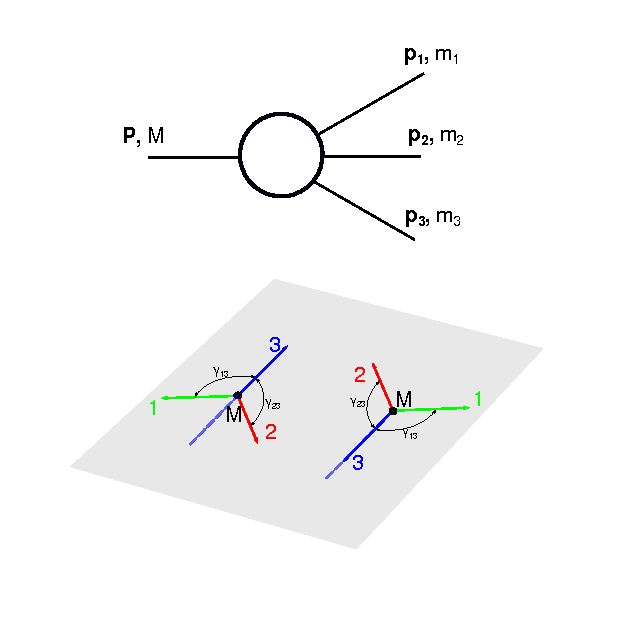
\includegraphics[]{pizerodecay.pdf}
\label{fig:pizdecay}
\caption{Figure for convention of 3 Body decay.}
\end{figure}

The physics of the 3-body decay can be completely described by the 4-vector relation,

\begin{equation}
p^\mu = p^\mu_1 + p^\mu_2 + p^\mu_3,
\label{eq:dalitz_fourvec}
\end{equation}
where in our decay,

\begin{equation}
p^\mu = \{M_\Delta,\vec{0}\}
\end{equation}

\begin{equation}
p^\mu_1 = \{E_\gamma,\vec{p}_\gamma\}
\end{equation}

\begin{equation}
p^\mu_2 = \{E_{e^-},\vec{p}_{e^-}\}
\end{equation}

\begin{equation}
p^\mu_3 = \{E_{e^+},\vec{p}_{e^-}\},
\end{equation}
which are given in the rest frame of the decay particle.


2-body decays are completely determined by energy and momentum conservation whereas 3-body decays have additional degrees of freedom. The phase space of a 3-body decay are best described by what is referred to as a Dalitz plot. There are 12 d.o.f. from the momentum vectors of 3 particles. Since the 3-body decay must occur within a plane we can remove 3 d.o.f. by conveniently selecting $p_{i,z} = 0$, 3 d.o.f. from energy momentum relations, 3 d.o.f. from momentum conservation, and 1 d.o.f. by noticing rotations in the x-y plane do not change the result. There are only two degrees of freedom that completely determine the system. In a Dalitz plot these variables are the invariant masses of two particles,

\begin{equation}
m^2_{12} = (p^\mu_1 + p^\mu_2)^2 = (p^\mu - p^\mu_3)^2 = M^2 + m_3^2 - 2ME_3
\label{eq:dalitz_m12}
\end{equation}

\begin{equation}
m^2_{23} = (p^\mu_2 + p^\mu_3)^2 = (p^\mu - p^\mu_1)^2 = M^2 + m_1^2 - 2ME_1
\label{eq:dalitz_m23}
\end{equation}

\begin{equation}
m^2_{13} = (p^\mu_1 + p^\mu_3)^2 = (p^\mu - p^\mu_2)^2 = M^2 + m_2^2 - 2ME_2.
\label{eq:dalitz_m13}
\end{equation}

Only two of these invariant masses are required to fully simulate the entire 3-body decay, where as the remaining invariant mass is determined by energy conservation, 

\begin{equation}
m^2_{12} + m^2_{23} + m^2_{13} = M^2 + \sum_i m_i^2.
\label{eq:dalitz_conserve}
\end{equation}


In our simulation the indicies are defined to each particle as such: 1$\leftrightarrow~e_-$, 2$ \leftrightarrow e^+$, and 3$ \leftrightarrow \gamma$. The invariant masses $m_{13}$ and $m_{23}$ are randomly generated and $m_{12}$ is given by Eq.~\ref{eq:dalitz_conserve}. The space in which $m_{13}$ and $m_{23}$ covers is generated uniformly. If $m_{12} \leq 0$ then the event is skipped as it did not meet the conservation criteria. The energies of each particle, $E_i$, can be solved for in Eq's~\ref{eq:dalitz_m12} \ref{eq:dalitz_m13} \ref{eq:dalitz_m23}. Also, the magnitude of the momentum $p_i$ is given by,

\begin{equation}
p_i^2 = E_i^2 - m_i^2.
\end{equation}

The angle of emission in the plane of the decay is fixed by these quantities. Modifying Eq.~\ref{eq:dalitz_fourvec}, we can solve for the angles between two particles $\gamma_{13}$ and $\gamma_{23}$, as defined in in Fig.~\ref{fig:pizdecay};

\begin{equation}
\cos(\gamma_{23}) =  \frac{2E_\gamma E_{e^+} + 2M_{\pi^0}E_{e^-} -M_{\piz}^2}{2p_{\gamma}p_{e^+}}
\end{equation}

\begin{equation}
\cos(\gamma_{13}) =  \frac{2E_\gamma E_{e^-} + 2M_{\piz}E_{e^+} -M_{\piz}^2}{2p_{\gamma}p_{e^-}}.
\end{equation}

The entire 4-vector of each particle, in the rest frame of the $\piz$, can be described in the plane of the decay. The axis along the decaying $\gamma$ must align with the momentum vector of the $\piz$ in the center of mass frame, by conservation of momentum. The direction of decay of the $\gamma$ has no preference and may decay forwards or backwards with respects to the incoming $\piz$ momentum, as illustrated in Fig.~\ref{fig:pizdecay}. Due to the symmetry along this same axis, the plane angle may be randomly oriented around the $\piz$ axis. In the simulation the angle of the plane is randomly rotated and half of the time the $\gamma$ decays forward and vice versa. 

The rest frame of the $\piz$ is defined by its momentum in the COM frame of the heavy ion collision where the Lorentz factor $\beta_{\piz}$ is given by the momentum and total energy of the pion,
\begin{equation}
\beta_{\piz} = \frac{ p_{\piz} }{E_{\piz}}.
\end{equation}

We assume the pion emission in the COM system is isotropic. Two Lorentz boosts are relevant in this simulation. First, the Lorentz boost from the rest frame of the pion to the COM of the h.i.c. Secondly from the COM system to the Lab frame which is defined by the Lorentz boost factor $\beta_{\mathrm{COM}}$, 

The resolution and acceptance of the TPC may smear or shift the $\elec$ and $\postr$ momentum distribution. We use the theoretically calculated momentum distribution in the lab frame as an input into the MC simulation of the TPC. The simulated spectra from the TPC is given in Fig.~ . The peak position has shifted significantly due systematic shifts in the momentum resolution. 






\end{document}

